\section{Homogeneous quadratics in $n$ variables}\label{sec:part1}
In this section we consider the case when
\[
	S = \{(x_1,\ldots,x_n) \mid Q(x_1,\ldots,x_n) = 0\}
\]
where $Q$ is a homogeneous quadratic. In order to compute $\Phi(\IND_S)$, we must determine $|\ker \lambda \cap S|$ for given $\lambda \in V^*$. If we think of elements of $V$ as column vectors, then elements $\lambda \in V^*$ can be thought of as row vectors, with
\[
	\ker \lambda = \langle \lambda \rangle^\bot = \{x \in V \mid \lambda x =0\}.
\]

We begin with an illustrative example over the reals before considering the situation over $\F_p$. Let $Q = 3x_1^2 + 3x_2^2 - 2x_3^2$. The conic $S = \{Q = 0\}$ is depicted in Figure~\ref{fig:conic-with-plane}.
\begin{figure}[h]
	\centering
	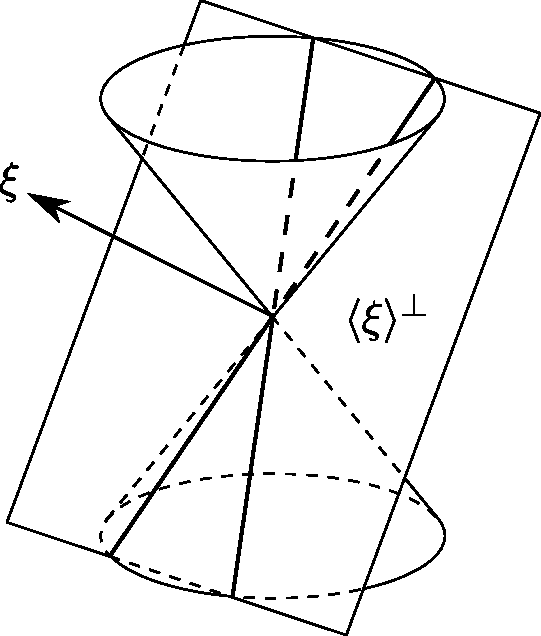
\includegraphics[width=0.6\linewidth]{conic-with-plane}
	\caption{}
	\label{fig:conic-with-plane}
\end{figure}
The intersection $\langle \lambda \rangle^\bot \cap S$ has three possible shapes:
\begin{itemize}
	\item a pair of lines intersecting at the origin (which is the case depicted with $\lambda = (0,-2,1)$),
	\item the origin alone (e.g. $\lambda = (0,0,1)$), and
	\item a single line, which happens when $\langle \lambda \rangle^\bot$ is tangent to the conic (e.g. $\lambda = (0,-\sqrt{3},\sqrt{2})$).
\end{itemize}
In fact, the set of $\lambda$ such that $\langle \lambda \rangle^\bot$ is tangent to the conic is given by
\[
	\left\{ \lambda = (\lambda_1,\lambda_2,\lambda_3) \mid \frac{1}{3} \lambda_1^2 + \frac{1}{3} \lambda_2^2 - \frac{1}{2} \lambda_3^2 = 0 \right\} \subset V^*.
\]
This is a conic in $V^*$, and it is dual to our original conic in a sense that we will soon explain. Let us we write $Q^*$ for the equation of this dual conic. Observe that $Q^*(0,-2,1) > 0$ while $Q^*(0,0,1) < 0$. It turns out that the sign of $Q^*(\lambda)$ is all one needs to classify the intersection $\langle \lambda \rangle^\bot \cap S$. Equivalently, one needs only consider the existence of square-roots of $Q^*(\lambda)$---a notion which, unlike ``sign,'' still makes sense over $\F_p$.

Now we consider the general situation in $n$ variables over a field $k$. We will require that $\operatorname{char} k \neq 2$, and that the product of two non-squares in $k$ is a square. The fields $\Q$, $\R$, and $\F_p$ for $p>2$ are examples. To a homogeneous quadratic
\[
	Q = \sum_{1 \leq i \leq j \leq n} c_{i,j} x_i x_j 
\]
we associate the $n\times n$ matrix $A$ whose entries are given by
\[
	a_{i,j} = \begin{cases}
		{c_{i,j}}/{2} & \text{if } i < j,\\
		c_{i,j} & \text{if } i = j, \text{ and}\\
		{c_{j,i}}/{2} & \text{if } i > j.
	\end{cases}
\]
Then, if $x = (x_1,\ldots,x_n)^\top$, we have
\[
	Q(x) = x^\top A x.
\]
The conic $S = \{Q = 0\}$ is \emph{non-degenerate} if the matrix $A$ is invertible. We will assume that this is the case.

\begin{defn}
	The \emph{orthogonal group of $A$}, denoted $O(A)$, is defined to be
	\[
		O(A) \coloneqq \{ g \in GL(V) \mid g^\top A g = A\}.
	\]
	Also define
	\[
		kO(A) \coloneqq \{ cg \mid c\in k, g\in O(A)\}.
	\]
\end{defn}

We are interested in this group because elements of $kO(A)$ map $S$ to itself.
\begin{defn}
	A group $G$ acts \emph{transitively} on a set $X$ if for all $a,b\in X$, there exists $g\in G$ such that $g\cdot a = b$. Equivalently, the only orbit of the action is the entirety of $X$.
\end{defn}

\begin{prop}\label{prop:OA-transitive-action}
	The group $kO(A)$ acts transitively on each of the following sets:
	\begin{enumerate}
		\item $S_0(A) \coloneqq \{x \in V \mid x\neq 0, x^\top A x = 0\}$,
		\item $S_+(A) \coloneqq \{ x\in V \mid x^\top A x \text{ is a nonzero square in } k\}$, and
		\item $S_-(A) \coloneqq \{ x\in V \mid x^\top A x \text{ is not a square in } k\}$.
	\end{enumerate}
\end{prop}
\begin{proof}
	If $u,v\in V$ belong to the same set above, we can assume $u^\top A u = v^\top A v$ (as it can be achieved by scaling). This relies on our assumption that the quotient of two non-squares is a square in $k$.
	
	If $u$ and $v$ are linearly dependent then the result is immediate, so suppose otherwise. Take a basis $\{u,v,e_3,\ldots,e_n\}$ and apply Gram-Schmidt to it, obtaining an orthogonal basis $\{u, w_2, w_3, \ldots,w_n\}$. Now consider the basis
	\[
		\{u,v,w_3,\ldots,w_n\}
	\]
	which has the property that
	\[
		w_i^\top A u = w_i^\top A v = w_i^\top A w_j = 0 \text{ for all } i \neq j, \text{ and }\\
		u^\top A u = v^\top A v.
	\]
	It is straightforward to verify that the linear transformation which interchanges $u$ and $v$ while fixing $w_3,\ldots,w_n$ is an element of $O(A)$.
\end{proof}

Note that left-multiplication by an element $g \in O(A)$ on $V$ induces right-multiplication by $g^{-1}$ on $V^*$.

Now suppose that $\lambda^\top,\lambda'^\top$ both belong to $S_0(A^{-1})$ (the following argument applies for the other two sets in Proposition \ref{prop:OA-transitive-action} as well). Then there exists $g \in O(A^{-1})$ such that $g \lambda^\top = \lambda'^\top$. If $\lambda x = 0$, then
\[
	\lambda' (g^\top)^{-1} x = \lambda x = 0
\]
and thus $(g^\top)^{-1}$ maps $\langle \lambda \rangle^\bot$ to $\langle \lambda' \rangle^\bot$. Moreover, since $g \in O(A^{-1})$, inverting the identity $g^\top A^{-1} g = A^{-1}$ shows that $(g^\top)^{-1} \in O(A)$.

Thus we get a map
\[
	(g^\top)^{-1} \colon S \cap \langle \lambda \rangle^\bot \to S \cap \langle \lambda' \rangle^\bot
\]
which is a bijection.

Specializing back to $k=\F_p$ for $p>2$ a prime, we conclude that $\Phi(\IND_S)$ assumes only a few values: specifically, it has the form
\begin{equation}\label{eq:FT-quadratic-constants-TBD}
	\Phi(\IND_S)(\lambda) = \begin{cases}
		\Phi(\IND_S)(0) & \text{if } \lambda = 0,\\
		N_0 & \text{if } \lambda \in S_0(A^{-1}),\\
		N_+ & \text{if } \lambda \in S_+(A^{-1}), \text{ and}\\
		N_- & \text{if } \lambda \in S_-(A^{-1}),
	\end{cases}
\end{equation}
for constants $\Phi(\IND_S)(0), N_0, N_+, N_-$ to be determined. Let $Q^*$ be the quadratic given by
\[
	Q^*(\lambda) = \lambda A^{-1} \lambda^\top.
\]
Then the above equivalently states that for nonzero $\lambda$, the value of $\Phi(\IND_S)(\lambda)$ depends only on the number of square roots of $Q^*(\lambda)$.

Now we compute the constants in \eqref{eq:FT-quadratic-constants-TBD}. It is a well-known fact (see for example \cite[Prop.~42:1]{omeara}) that there exists an invertible $n\times n$ matrix $P$ such that $P^\top A P$ is diagonal. The matrix $P$ defines a change of coordinates, where in the new coordinates the equation of the quadric is
\[
x^\top P^\top A P x = 0.
\]
Since $P^\top A P$ is diagonal, this equation takes the form
\[
c_1 x_1^2 + c_2 x_2^2 + \cdots + c_n x_n^2 = 0
\]
where all the $c_i$ are nonzero because we assumed $A$ to be invertible.

Fix a non-square $r\in \F_p$. For each $c_i$, either $c_i$ is a square or $c_i / r$ is a square. By scaling the coordinates as needed, we can assume that each $c_i$ is either $1$ or $r$.

There exists an $a\in\F_p$ such that $a^2 + 1$ is a non-square. Suppose that for distinct $i,j\in\{1,\ldots,n\}$ the coefficients of $x_i$ and $x_j$ are both $r$. We can apply the invertible transformation which replaces $x_i$ by $ax_i + x_j$ and $x_j$ by $x_i - ax_j$ in the equation for the quadric, and this turns the expression $rx_i^2 + rx_j^2$ into $r(a^2 + 1)x_i^2 + r(a^2+1)x_j^2$. As the product of two non-squares, these new coefficients are squares. Hence we may assume that they are equal to $1$.

This shows that we can reduce to the two following forms:
\begin{align}
x_1^2 + x_2^2 + \cdots + x_n^2 &= 0\text{ or} \tag{Q1}\label{eq:Q1}\\ 
rx_1^2 + x_2^2 + \cdots + x_n^2 &= 0. \tag{Q2}\label{eq:Q2}
\end{align}
In Appendix \ref{sec:recursion-for-quadratic-solns} we give recursions $f_n, g_n$ for computing the number of solutions to such equations. We conclude this section by giving an example of how to compute the constants in \eqref{eq:FT-quadratic-constants-TBD} from $f_n$ and $g_n$.

\begin{example}
	Suppose our equation is to the form \eqref{eq:Q1} and $-1$ is a square mod $p$. Then $\Phi(\IND_S)(0)$ is the total number of points on the quadric, which in this case is $f_n (0)$:
	\[
		\Phi(\IND_S)(0) = f_n(0).
	\]
	To compute $N_0$, observe that \eqref{eq:Q1} is equivalent to
	\[
		-x_1^2 + x_2^2 + \cdots + x_n^2 = 0
	\]
	because $-1$ is a square. Consider $\lambda = (1,1,0,0,\ldots,0)$. Its kernel is the hyperplane $\{x_1 + x_2 = 0\}$. Substituting $x_1 = -x_2$ into the above gives
	\[
	x_3^2 + \cdots + x_n^2 = 0.
	\]
	This has $p f_{n-2}(0)$ solutions in the variables $x_2,\ldots,x_n$. Thus
	\[
	N_0 = \frac{p^2 f_{n-2}(0) - f_n(0)}{p-1}.
	\]
	To compute $N_+$, consider $\lambda = (1,0,0,\ldots,0)$ whose kernel is the hyperplane $\{x_1 = 0\}$. Substituting this into \eqref{eq:Q1} gives
	\[
	x_2^2 + x_3^2 \cdots + x_n^2 = 0
	\]
	which has $f_{n-1}(0)$ solutions in the variables $x_2,x_3,\ldots,x_n$, and thus
	\[
	N_+ = \frac{p f_{n-1}(0) - f_n(0)}{p-1}.
	\]
	Finally, to compute $N_-$, we note that \eqref{eq:Q1} is also equivalent to the quadric
	\[
		rx_1^2 + rx_2^2 + x_3^2 + \cdots + x_n^2 = 0
	\]
	and we can take $\lambda = (1,0,0,\ldots,0)$ and consider the intersection of its kernel with this quadric. Setting $\{x_1 = 0\}$ gives the equation
	\[
		rx_2^2 + x_3^2 + \cdots + x_n^2 = 0
	\]
	which has $g_{n-1}(0)$ solutions, and hence
	\[
		N_- = \frac{pg_{n-1}(0) - f_n(0)}{p-1}.
	\]
	Actually, because $n$ is even, $f_{n-1}(0) = g_{n-1}(0)$ (c.f. Appendix \ref{sec:recursion-for-quadratic-solns}). So we in fact have $N_+ = N_-$.
\end{example}